\documentclass[conference,compsoc]{IEEEtran}
\usepackage{amsmath}
\usepackage{amsthm}
\usepackage{complexity}
\usepackage{amssymb}
\usepackage{graphicx}
\usepackage{hyperref}
\usepackage{tikz}
\usepackage{algorithm, algorithmic}
\usepackage{lipsum}
\usetikzlibrary{backgrounds}
\setlength{\parskip}{0 em}
\hypersetup{
    colorlinks=true,
    linkcolor=blue,
    filecolor=magenta,      
    urlcolor=blue,
}
\urlstyle{same}

\ifCLASSOPTIONcompsoc
  % IEEE Computer Society needs nocompress option
  % requires cite.sty v4.0 or later (November 2003)
  \usepackage[nocompress]{cite}
  
  
\else
  % normal IEEE
  \usepackage{cite}
\fi

% correct bad hyphenation here
\hyphenation{op-tical net-works semi-conduc-tor}


\begin{document}
\title{An Evolutionary Approach to the Graph Bandwidth Problem}
\author{\IEEEauthorblockN{Maaz Saeed}
\IEEEauthorblockA{Dhanani School of Science\\and Engineering\\
Habib University\\
Karachi - 75290, Sindh, Pakistan\\
Email: @st.habib.edu.pk}
\and
\IEEEauthorblockN{Muhammad Usaid Rehman}
\IEEEauthorblockA{Dhanani School of Science\\and Engineering\\
Habib University\\
Karachi - 75290, Sindh, Pakistan\\
Email: mr04302@st.habib.edu.pk}
\and
\IEEEauthorblockN{Maham Shoaib Patel}
\IEEEauthorblockA{Dhanani School of Science\\and Engineering\\
Habib University\\
Karachi - 75290, Sindh, Pakistan\\
Email: mp04911@st.habib.edu.pk}}

\maketitle

\begin{abstract}
  The Graph Bandwidth Problem, is an NP-Complete, lesser researched, special case of 
  Quadratic Bottleneck Assignment problem. It is an optimization problem with the objective of 
  minimizing distance between a pair of vertices of a graph. Save a few research papers from the 
  20th century, the graph bandwidth problem has not enjoyed nearly the same spotlight in the world 
  of research as other combinatorial problems, including the likes of Traveling Salesman and Knapsack problems. 
  As students of Computational Intelligence, we found it imperative to explore the problem through the lens of 
  Evolutionary Algorithms. Since the problem is NP-hard and can not be solved in constant time, there is great potential 
  for a meta-heuristic approach. Our team aims to explore said potential by applying evolutionary 
  algorithms to graphs of varying sizes, and deliver a user-friendly application that accurately approximates solutions.
\end{abstract}
\textbf{Keywords:} Graph Theory, Graph Bandwidth, Evolutionary Algorithms

\IEEEpeerreviewmaketitle

\section{Introduction} 
The graph bandwidth is a well-studied problem in graph theory. It is a combinatorial optimzation problem where the objective 
is to minimize the maximum distance between two vertices of a graph by finding a suitable labelling $f: V(G) \to \{1, 2, \dots, n\}$.
There are two different forms of the bandwidth problem -- the bandwidth problem for graphs and the bandwidth problem for matrices. 
Both versions of the problem are closely related since the graph version of the problem can be reduced to the matrix version using 
the adjacency matrix of the graph. 
The problem can be visualized as placing the vertices of a graph at distinct integer points along the $x$-axis so that the 
length of the longest edge is minimized. 

The inception of the matrix bandwidth problem occurred in the 1950s when structural engineers 
attempted to analyze steel frameworks by their structural matrices via computerized manipulation. The term 'bandwidth' 
was birthed as the engineers had endeavoured to discover a matrix in which all the non-zero elements 
lay withing a narrow 'band'. The inspiration for this came from operations such as 
inversion or finding determinant in as little time as possible.

In 1962, similar to this approach, L.H Harper, and A.W Hales conceived the bandwidth, 
and bandwidth sum. They used edge differences to represent single errors in a 6-bit picture code, 
in a hypercube, where it's vertices were words of the code \cite{10.2307/2946514}. Some time after this, 
R.R Kohrfage initialized his work on the graph bandwidth problem \cite{ccdg1982}. Finally, F. Harary 
published the problem, as we know it today, officially \cite{https://doi.org/10.1002/bimj.19660080427}.

\subsection{Formal Definition} \label{intro}
In more formal terms, 
the mapping $f$ is defined as $f: V(G) \to \{1, 2, \dots, n\}$, where $n = |V|$. This is also called 
a \emph{proper numbering} of the graph $G$.\cite{Lee2016} Therefore, 
we can think of these mappings as essentially labelling or numbering of the vertices. The bandwidth of a numbering $f$
is defined as:
\begin{equation}
B_f(G) = \max_{uv \in E(G)}\{|f(u) - f(v)|\}
\end{equation}

The bandwidth of the graph $G$ is given by the bandwidth of the best possible numbering:
\begin{equation}
  B(G) = \min \{B_f(G): f \; \text{is a numbering of }  G\}
\end{equation}
Bandwidths can be computed using any integer mapping, however, to make our implementation 
easier, we will be restricting ourselves to working with proper numberings only.

There exist several known mathematical bounds that relate the bandwidth of a graph 
to various graph theoretic properties. For example, it is a simple exercise to prove that 
\[B(G) = n - 1\] where $G$ is a complete graph of the form $K_n$. Similarly, there are also bounds 
relating the chromatic number and diameter with the bandwidth of the graph.  \cite{ccdg1982}

\subsection{NP-Completeness of the bandwidth problem}

The bandwidth problem itself is a special case of the quadratic bottleneck assignment problem, which is known to be 
$\NP$-hard. It is also known that the bandwidth problem is $\NP$-hard to approximate which makes it impossible to find 
an $O(1)$-approximation algorithm for the bandwidth problem. 

Historically, there have been endeavours to decrease (see \cite{10.1145/800195.805928}, \cite{sparse}), or minimize 
(see \cite{chen}, \cite{chen2}) 
the bandwidth of large, spares matrices, effectively, by permuting rows and columns. 
This has been translated to graph theory by Harary (see \cite{1973141}). 
Papadimitriou proved that the minimization of the bandwidth of a matrix is an 
\NP-complete problem. \cite{papadimitriou_1976}

There are several heuristic algorithms for the bandwidth problems such as the Cuthill-McKee algorithm, and the 
Gibbs-Poole-Stockmeyer algorithm.  Heuristic approaches are of interest to us since they will give us an 
idea ad to how we can design appropriate meta-heuristic techniques to solve the bandwidth problem. 

\section{Evolutionary Algorithms}
Evolutionary Algorithms (also known as Genetic Algorithms) is a term referring to a 
family of algorithms based on the evolution we see around us, in nature. By mimicking learning, 
natural selection, reproduction, we can produce solutions for various search and optimization problems. 
This concept of evolving algorithms enables us to bypass the setbacks of traditional search / optimization algorithms.

\subsection{Darwinian Evolution}
Evolutionary Algorithms are derived of a simplified Darwinian evolution. The principles of such a cycle can be as such:
\begin{enumerate}
    \item \textbf{Variation} - Individual members of a given population may have differing attributes 
    from one another, for example, physical appearance.
    \item \textbf{Inheritance} - Offspring resemble their parents to certain extents. 
    In this manner, traits are passed down from one generation to another; unrelated individuals are less likely to have common traits, as 
    compared to them with their family trees.
    \item \textbf{Selection} - Nature follows 'survival of the fittest' ideology. Individuals that 
    are better able to locate and make use of resources compared to their peers, are more likely to survive in their respective environments. 
\end{enumerate}
In accordance with these principals, results that we obtain from our algorithm may or may not resemble those of 
previous iterations. With careful manipulation of parameters, solutions produced by our code can be ranked 
higher or lower than others.
\subsection{Analogies}
Where Darwinian evolution maintains a population of individual solutions, genetic algorithms maintain 
\textbf{individuals} - a population of candidate solutions \cite{Wiransky-GA}. The theory behind these 
algorithms is that solutions are produced, and improved upon, by iteratively re-producing newer generations of solutions.

The various components of an evolutionary algorithm are as follows:
\begin{enumerate}
    \item \textbf{Genotype} - In nature, genotypes are collections of genes. When two individuals procreate, a mixture of genes 
    from both, will make up the chromosomes of the offspring. In code, these \textbf{chromosomes} 
    can be expressed, for example, as strings in binary. 
    \item \textbf{Population} - Population refers to the collection of chromosomes. At any given moment, the 
    algorithm will maintain a population of individuals - candidate solutions for the problem that is being attempted 
    to be solved. In a nutshell, it is the current generation, which will be replaced by the next generation of offspring. 
    \item \textbf{Fitness Function} - a function used to evaluate individuals in a given population. Individuals 
    that produce better results, will be more favoured when it comes to selection for breeding of newer generations. As this cycle runs, 
    individuals display continuous improvement until a satisfactory solution to our problem is found, at which point we can terminate the operation.
    \item \textbf{Selection} - After individuals are evaluated and awarded a \textit{fitness value}, 
    the best among them are chosen to breed and produce the newer generation. It is important to note 
    that individuals with lower scores are still selected, but with lower probabilities, so as to not 
    cause extinction of their respective attributes.
    \item \textbf{Crossover} - refers to the mixing of chromosomes of the two parent individuals 
    that were paired in the selection process to produce two new chromosomes (offspring). This process is also known as recombination.
    \item \textbf{Mutation} - fulfills the purpose of periodically (at random; not in a set pattern) refreshing 
    the population. This introduction of new patterns in the chromosomes encourages the algorithm to search in unexplored areas, rather than 
    just exploiting what it has already chartered. The mutation may occur as random changes in chromosomes, for example, in binary string 
    representation, a single bit may be switched.
\end{enumerate}
\begin{figure}[h]
  \centering
  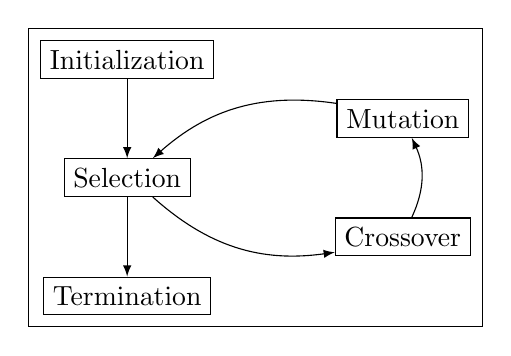
\begin{tikzpicture}[framed]
  \node[rectangle, draw=black] (A) at (0,0) {Initialization};
  \node[rectangle, draw=black] (B) at (0,-1.5) {Selection};
  \node[rectangle, draw=black] (C) at (0, -3) {Termination};
  \node[rectangle, draw=black] (D) at (3.5, -0.75) {Mutation};
  \node[rectangle, draw=black] (E) at (3.5, -2.25) {Crossover};
  \draw[-latex] (A) -- (B);
  \draw[-latex] (B) -- (C);
  \draw[-latex] (B) to[bend right=25] (E);
  \draw[-latex] (D) to[bend right=25] (B);
  \draw[-latex] (E) to[bend right=25] (D);
  \end{tikzpicture}
  \caption{Flowchart of Evolutionary Algorithms}
\end{figure}
\setlength{\parskip}{0 em}
\section{Implementation Details}
\subsection{Population Represenation}
In our implementation, an individual chromosome in our population 
is stored in the form of key-value pairs\footnote{In Python, this is implemented 
as a dictionary}, where the key is the vertex and the value is the integer label 
of the vertex. 
\setlength{\parskip}{0.4 em}

The population can be expressed as the set \[\{(v_i, f(v_i)): \; v_i \in V(G)\}\]
where $v_i$ is a vertex in graph $G$ and $f(v_i)$ is the integer label of the 
vertex. To initialize the population, we generated individuals using randomized numberings. 
Therefore, each individual is a proper numbering of the graph (see Section \ref{intro}). While storing the numberings, 
we also compute the fitness of each individual (see Section \ref{fit}) and store it along with 
each individual. 

\setlength{\parskip}{0 em}
\subsection{Fitness Function} \label{fit}
The fitness function in our implementation was derived simply from the problem. Each individual was a proper numbering 
of the graph, and therefore, each individual had a corresponding bandwidth as described in Section \ref{intro}. Therefore, 
we simply iterated over the edges of the graph and then found the maximum value. We can also say that we found 
the bandwidth $B_f(G)$ for a single numbering/ordering $f$. 

\begin{algorithm}
\caption{Fitness Function}
\begin{algorithmic}[1]
  \renewcommand{\algorithmicrequire}{\textbf{Input:}}
  \renewcommand{\algorithmicensure}{\textbf{Output:}}
  \REQUIRE A chromosome
  \ENSURE  The fitness (bandwidth) of the chromosome
  \\ \textit{Initialize edge map: }
  \STATE $A \leftarrow \{(uv): 0\} \; \; \; \forall uv \in E(G)$
  \\ \textit{Compute fitness: }
  \FOR {each $uv \in E(G)$}
  \STATE $A[uv] \leftarrow \lvert f(u) - f(v) \rvert$
  \ENDFOR
  \STATE fitness $\leftarrow \max(A)$
  \RETURN fitness 
\end{algorithmic}
\end{algorithm}

\subsection{Selection}
\lipsum[1]
\subsection{Crossover \& Mutation}
We performed a two-point crossover in order to bring genetic diversity to the 
population. All offspring was generated using the crossover operation, i.e. no offspring 
were copies of their parent chromosomes. A generic crossover 
method could not be used since the numbering had to be unique\footnote{similar to the Travelling Salesperson Problem}.

\begin{algorithm}
\caption{Crossover}
\begin{algorithmic}
  
\end{algorithmic}
\end{algorithm}
\section{Experimental Analysis}
\subsection{Testing Methods}
\subsection{Results}
\section{Conclusion}
The conclusion goes here.



% % use section* for acknowledgment
% \ifCLASSOPTIONcompsoc
%   % The Computer Society usually uses the plural form
%   \section*{Acknowledgments}
% \else
%   % regular IEEE prefers the singular form
%   \section*{Acknowledgment}
% \fi






\bibliographystyle{ieeetr}
\bibliography{refs.bib}

\end{document}
